% answers.tex —— 2015 年·浙江卷·理科 · 参考答案与详细解析片段
% 由 tools/generate_projects.py 依来源总账自 2015/2015_数学真题_浙江理_试题.md + 2015/2015_数学真题_浙江理_解析正文.md + 2015/2015_数学真题_浙江理_答案要点.md 生成，勿手改（改源 MD 后重跑）

\begin{gktip}
固定原卷不附参考答案（证据等级 D）；以下推导由项目独立完成，并经独立角色盲核，不作为官方解析。
\end{gktip}

\begin{answer}
\gksolhead{1}{集合运算}

\textbf{题目}：

已知集合 \(P=\{x\mid x^2-2x\geqslant0\}\)，\(Q=\{x\mid 1<x\leqslant2\}\)，则 \((\complement_{\mathbf{R}}P)\cap Q=\)（　）

(A) \([0,1)\)　(B) \((0,2]\)　(C) \((1,2)\)　(D) \([1,2]\)

\Needspace{4\baselineskip}
\textbf{解析}

\Needspace{5\baselineskip}
由 \(x^2-2x\geqslant0\) 得 \(x(x-2)\geqslant0\)，故
\nopagebreak[4]
\[
P=(-\infty,0]\cup[2,+\infty),\qquad \complement_{\mathbf{R}}P=(0,2).
\]
\Needspace{5\baselineskip}
又 \(Q=(1,2]\)，求交得
\nopagebreak[4]
\[
(\complement_{\mathbf{R}}P)\cap Q=(0,2)\cap(1,2]=(1,2).
\]

故选 (C)。

（验证：取 \(x=\dfrac32\in Q\)，\(x^2-2x=-\dfrac34<0\)，在 \(\complement_{\mathbf{R}}P\) 中；取 \(x=2\)，\(x^2-2x=0\)，属于 \(P\) 而不在补集中；端点 \(x=1\notin Q\)，故交集左端开、右端开。）

\gkanswer{答案：C}

\end{answer}
\begin{answer}
\gksolhead{2}{三视图与体积}

\textbf{题目}：

某几何体的三视图如图所示（单位：\(\mathrm{cm}\)），则该几何体的体积是（　）
\nopagebreak[4]
\begin{center}% f2015zjl_q02_views.tex — 2015 年高考数学·浙江卷·理科 第 2 题（三视图）
%
% 【来源】`.work/phase3-b19/source/2015浙江理.pdf`（SHA-256
%   801150f0a6d440ac967813d264face6d48b6ee9c69cc20f1c9d6b2b38dec2e9f），
%   第 1 页（合订本页 989）；内容对象 5。逐路径实测见
%   `.work/phase3-b19/figure-inventory.md`。
%
% 【坐标口径】源 PDF 用户空间（原点左下、y 向上）。本图本地坐标
%   (x, y) = (x_page − 145.498, y_page − 383.098)，1 单位 = 1 TeX pt。
%   路径坐标逐点照录内容流（含三次贝塞尔控制点）。
%
% 元素计数：30 条路径（三视图轮廓/对角线/尺寸线/箭头）＋7 个标签
\begin{tikzpicture}[x=1pt, y=1pt,
    every node/.style={inner sep=0pt, font=\fontsize{10.5pt}{12.6pt}\selectfont}]
  \draw[line width=0.398pt] (0.0000,9.3547)   -- (62.3630,71.7177);
  \draw[line width=0.398pt] (0.0000,71.7180)   -- (62.3630,9.3550);
  \draw[line width=0.398pt] (0.0000,165.2630)   -- (62.3630,165.2630);
  \draw[line width=0.398pt] (93.5450,165.2630)   -- (155.9080,165.2630);
  \draw[line width=0.398pt] (0.0000,6.2363)   -- (0.0000,0.0003);
  \draw[line width=0.398pt] (62.3633,6.2363)   -- (62.3633,0.0003);
  \draw[line width=0.398pt] (65.4817,9.3547)   -- (71.7177,9.3547);
  \draw[line width=0.398pt] (65.4817,71.7180)   -- (71.7177,71.7180);
  \draw[line width=0.398pt] (65.4817,102.8996)   -- (71.7177,102.8996);
  \draw[line width=0.398pt] (65.4817,165.2630)   -- (71.7177,165.2630);
  \draw[line width=0.398pt] (65.4817,227.6263)   -- (71.7177,227.6263);
  \draw[line width=0.398pt] (24.9454,3.1184)   -- (3.5864,3.1184);
  \fill[line width=1.0pt] (0.0000,3.1184)   .. controls (1.0630,2.9194) and (2.7900,2.3214) .. (3.9850,1.6244)   -- (3.9850,4.6124)   .. controls (2.7900,3.9154) and (1.0630,3.3174) .. (0.0000,3.1184);
  \draw[line width=0.398pt] (68.5995,34.3001)   -- (68.5995,12.9411);
  \fill[line width=1.0pt] (68.5996,9.3547)   .. controls (68.7986,10.4177) and (69.3966,12.1447) .. (70.0936,13.3397)   -- (67.1056,13.3397)   .. controls (67.8026,12.1447) and (68.4006,10.4177) .. (68.5996,9.3547);
  \draw[line width=0.398pt] (68.5995,46.7725)   -- (68.5995,68.1315);
  \fill[line width=1.0pt] (68.5996,71.7179)   .. controls (68.4006,70.6549) and (67.8026,68.9279) .. (67.1056,67.7329)   -- (70.0936,67.7329)   .. controls (69.3966,68.9279) and (68.7986,70.6549) .. (68.5996,71.7179);
  \draw[line width=0.398pt] (68.5995,127.8451)   -- (68.5995,106.4861);
  \fill[line width=1.0pt] (68.5996,102.8997)   .. controls (68.7986,103.9627) and (69.3966,105.6897) .. (70.0936,106.8847)   -- (67.1056,106.8847)   .. controls (67.8026,105.6897) and (68.4006,103.9627) .. (68.5996,102.8997);
  \draw[line width=0.398pt] (68.5995,140.3175)   -- (68.5995,161.6765);
  \fill[line width=1.0pt] (68.5996,165.2629)   .. controls (68.4006,164.1999) and (67.8026,162.4729) .. (67.1056,161.2779)   -- (70.0936,161.2779)   .. controls (69.3966,162.4729) and (68.7986,164.1999) .. (68.5996,165.2629);
  \draw[line width=0.398pt] (68.5995,190.2084)   -- (68.5995,168.8494);
  \fill[line width=1.0pt] (68.5996,165.2630)   .. controls (68.7986,166.3260) and (69.3966,168.0530) .. (70.0936,169.2480)   -- (67.1056,169.2480)   .. controls (67.8026,168.0530) and (68.4006,166.3260) .. (68.5996,165.2630);
  \draw[line width=0.398pt] (68.5995,202.6809)   -- (68.5995,224.0399);
  \fill[line width=1.0pt] (68.5996,227.6263)   .. controls (68.4006,226.5633) and (67.8026,224.8363) .. (67.1056,223.6413)   -- (70.0936,223.6413)   .. controls (69.3966,224.8363) and (68.7986,226.5633) .. (68.5996,227.6263);
  \draw[line width=0.398pt] (37.4179,3.1184)   -- (58.7769,3.1184);
  \fill[line width=1.0pt] (62.3633,3.1184)   .. controls (61.3003,3.3174) and (59.5733,3.9154) .. (58.3783,4.6124)   -- (58.3783,1.6244)   .. controls (59.5733,2.3214) and (61.3003,2.9194) .. (62.3633,3.1184);
  \draw[line width=0.398pt] (0.0000,9.3547)   -- (0.0000,71.7177)   -- (62.3630,71.7177)   -- (62.3630,9.3547)   -- cycle;
  \draw[line width=0.398pt] (0.0000,102.8996)   -- (62.3630,102.8996)   -- (62.3630,165.2626)   -- (31.1820,227.6266)   -- (0.0000,165.2626)   -- cycle;
  \draw[line width=0.398pt] (93.5450,102.8996)   -- (155.9080,102.8996)   -- (155.9080,165.2626)   -- (124.7270,227.6266)   -- (93.5450,165.2626)   -- cycle;

  \node[anchor=center] at (31.152,87.942) {正视图};  % 源中心 (176.65,471.04)
  \node[anchor=center] at (124.752,87.942) {侧视图};  % 源中心 (270.25,471.04)
  \node[anchor=center] at (31.152,-10.258) {俯视图};  % 源中心 (176.65,372.84)
  \node[anchor=center] at (68.602,195.692) {$2$};  % 源中心 (214.10,578.79)
  \node[anchor=center] at (68.602,133.342) {$2$};  % 源中心 (214.10,516.44)
  \node[anchor=center] at (68.602,39.742) {$2$};  % 源中心 (214.10,422.84)
  \node[anchor=center] at (31.202,2.342) {$2$};  % 源中心 (176.70,385.44)

\end{tikzpicture}
%
% 【自验结果】
%   探针：latexmk -pdfxe（待跑）。
\end{center}
\nopagebreak[4]
(A) \(8\,\mathrm{cm}^3\)　(B) \(12\,\mathrm{cm}^3\)　(C) \(\dfrac{32}{3}\,\mathrm{cm}^3\)　(D) \(\dfrac{40}{3}\,\mathrm{cm}^3\)

\Needspace{4\baselineskip}
\textbf{解析}

由三视图可知，该几何体下部是棱长为 \(2\) 的正方体，上部是底面为 \(2\times2\)、高为 \(2\) 的正四棱锥。俯视图中的两条对角线即四棱锥四条侧棱在底面上的投影。

\Needspace{5\baselineskip}
下部体积
\nopagebreak[4]
\[
V_1=2^3=8.
\]
\Needspace{5\baselineskip}
上部四棱锥体积
\nopagebreak[4]
\[
V_2=\frac13\cdot2^2\cdot2=\frac83.
\]
\Needspace{5\baselineskip}
故几何体体积
\nopagebreak[4]
\[
V=V_1+V_2=8+\frac83=\frac{32}{3}\ \left(\mathrm{cm}^3\right).
\]

故选 (C)。

（验证：正视图与侧视图均为「边长 2 的正方形上加高 2 的等腰三角形」——矩形高与三角形高各标一个「2」；俯视图为 \(2\times2\) 正方形加两条对角线，对角线交点即锥顶投影。若误把总高 \(4\) 当作锥高，会得干扰项 \(\dfrac{40}{3}\)。）

\gkanswer{答案：C}

\end{answer}
\begin{answer}
\gksolhead{3}{等差数列与等比中项}

\textbf{题目}：

已知 \(\{a_n\}\) 是等差数列，公差 \(d\) 不为零，前 \(n\) 项和是 \(S_n\)。若 \(a_3\)，\(a_4\)，\(a_8\) 成等比数列，则（　）

(A) \(a_1d>0\)，\(dS_4>0\)　(B) \(a_1d<0\)，\(dS_4<0\)　(C) \(a_1d>0\)，\(dS_4<0\)　(D) \(a_1d<0\)，\(dS_4>0\)

\Needspace{4\baselineskip}
\textbf{解析}

\Needspace{5\baselineskip}
设首项为 \(a_1\)、公差为 \(d\neq0\)。由 \(a_3\)，\(a_4\)，\(a_8\) 成等比数列得
\nopagebreak[4]
\[
a_4^2=a_3a_8,
\]
\Needspace{5\baselineskip}
即
\nopagebreak[4]
\[
(a_1+3d)^2=(a_1+2d)(a_1+7d).
\]
\Needspace{5\baselineskip}
展开整理：
\nopagebreak[4]
\[
a_1^2+6a_1d+9d^2=a_1^2+9a_1d+14d^2
\ \Longrightarrow\ 3a_1d+5d^2=0.
\]
\Needspace{5\baselineskip}
因 \(d\neq0\)，故
\nopagebreak[4]
\[
a_1=-\frac{5d}{3},\qquad a_1d=-\frac{5d^2}{3}<0.
\]
\Needspace{5\baselineskip}
又
\nopagebreak[4]
\[
S_4=4a_1+\frac{4\cdot3}{2}d=4\left(-\frac{5d}{3}\right)+6d=-\frac{2d}{3},
\]
\Needspace{5\baselineskip}
所以
\nopagebreak[4]
\[
dS_4=-\frac{2d^2}{3}<0.
\]

故选 (B)。

（验证：取 \(d=3\)，则 \(a_1=-5\)，数列为 \(-5,-2,1,4,\cdots\)；\(a_3=1\)，\(a_4=4\)，\(a_8=16\)，满足 \(4^2=1\times16\)；此时 \(a_1d=-15<0\)，\(S_4=-2\)，\(dS_4=-6<0\)。取 \(d=-3\) 结论相同。）

\gkanswer{答案：B}

\end{answer}
\begin{answer}
\gksolhead{4}{全称命题的否定}

\textbf{题目}：

命题“\(\forall n\in\mathbf{N}^*\)，\(f(n)\in\mathbf{N}^*\) 且 \(f(n)\leqslant n\)”的否定形式是（　）

(A) \(\forall n\in\mathbf{N}^*\)，\(f(n)\notin\mathbf{N}^*\) 且 \(f(n)>n\)　(B) \(\forall n\in\mathbf{N}^*\)，\(f(n)\notin\mathbf{N}^*\) 或 \(f(n)>n\)　(C) \(\exists n_0\in\mathbf{N}^*\)，\(f(n_0)\notin\mathbf{N}^*\) 且 \(f(n_0)>n_0\)　(D) \(\exists n_0\in\mathbf{N}^*\)，\(f(n_0)\notin\mathbf{N}^*\) 或 \(f(n_0)>n_0\)

\Needspace{4\baselineskip}
\textbf{解析}

\Needspace{5\baselineskip}
原命题为 \(\forall n\in\mathbf{N}^*\)，\(f(n)\in\mathbf{N}^*\) 且 \(f(n)\leqslant n\)。全称命题的否定是存在命题，且由德摩根律
\nopagebreak[4]
\[
\neg\bigl(f(n)\in\mathbf{N}^*\ \text{且}\ f(n)\leqslant n\bigr)
\equiv\ f(n)\notin\mathbf{N}^*\ \text{或}\ f(n)>n.
\]
\Needspace{5\baselineskip}
故否定形式为
\nopagebreak[4]
\[
\exists n_0\in\mathbf{N}^*,\qquad f(n_0)\notin\mathbf{N}^*\ \text{或}\ f(n_0)>n_0.
\]

故选 (D)。

（验证：取 \(f(n)=n+1\)，原命题为假；其否定应为真。取 \(n_0=1\)，\(f(1)=2>1\)，D 成立。若误选 C，「且」要求两个条件同时成立，而 \(2\in\mathbf{N}^*\)，C 为假。）

\gkanswer{答案：D}

\end{answer}
\begin{answer}
\gksolhead{5}{抛物线与面积比}

\textbf{题目}：

如图，设抛物线 \(y^2=4x\) 的焦点为 \(F\)，不经过焦点的直线上有三个不同的点 \(A\)，\(B\)，\(C\)，其中点 \(A\)，\(B\) 在抛物线上，点 \(C\) 在 \(y\) 轴上，则 \(\triangle BCF\) 与 \(\triangle ACF\) 的面积之比是（　）
\nopagebreak[4]
\begin{center}% f2015zjl_q05_parabola.tex — 2015 年高考数学·浙江卷·理科 第 5 题（抛物线与三点）
%
% 【来源】`.work/phase3-b19/source/2015浙江理.pdf`（SHA-256
%   801150f0a6d440ac967813d264face6d48b6ee9c69cc20f1c9d6b2b38dec2e9f），
%   第 1 页（合订本页 989）；内容对象 5。逐路径实测见
%   `.work/phase3-b19/figure-inventory.md`。
%
% 【坐标口径】源 PDF 用户空间（原点左下、y 向上）。本图本地坐标
%   (x, y) = (x_page − 509.212, y_page − 599.834)，1 单位 = 1 TeX pt。
%   路径坐标逐点照录内容流（含三次贝塞尔控制点）。
%
% 元素计数：10 条路径（x/y 轴＋箭头、上下两支抛物线、割线 C–B–A、CF/FB/FA）＋7 个标签
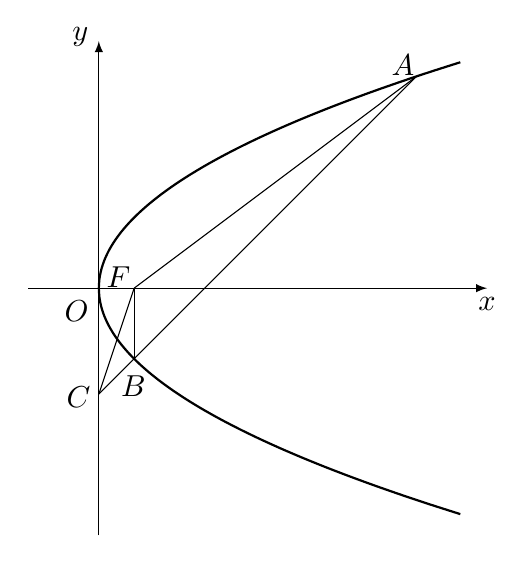
\begin{tikzpicture}[x=1pt, y=1pt,
    every node/.style={inner sep=0pt, font=\fontsize{10.5pt}{12.6pt}\selectfont}]
  \draw[line width=0.398pt] (0.0001,89.2920)   -- (162.2411,89.2920);
  \fill[line width=1.0pt] (165.8277,89.2920)   .. controls (164.7647,89.4910) and (163.0377,90.0890) .. (161.8427,90.7860)   -- (161.8427,87.7980)   .. controls (163.0377,88.4950) and (164.7647,89.0930) .. (165.8277,89.2920);
  \draw[line width=0.398pt] (25.5120,0.0002)   -- (25.5120,174.9972);
  \fill[line width=1.0pt] (25.5120,178.5838)   .. controls (25.3130,177.5208) and (24.7150,175.7938) .. (24.0180,174.5988)   -- (27.0060,174.5988)   .. controls (26.3090,175.7938) and (25.7110,177.5208) .. (25.5120,178.5838);
  \draw[line width=0.797pt] (25.5120,89.2920)   .. controls (25.5120,89.2920) and (25.6130,91.7500) .. (25.7390,92.6940)   .. controls (25.8650,93.6370) and (26.1670,95.1510) .. (26.4190,96.0950)   .. controls (26.6710,97.0390) and (27.1750,98.5530) .. (27.5530,99.4970)   .. controls (27.9300,100.4410) and (28.6370,101.9540) .. (29.1400,102.8980)   .. controls (29.6440,103.8420) and (30.5520,105.3560) .. (31.1810,106.3000)   .. controls (31.8100,107.2440) and (32.9200,108.7570) .. (33.6750,109.7010)   .. controls (34.4310,110.6450) and (35.7420,112.1590) .. (36.6230,113.1030)   .. controls (37.5040,114.0470) and (39.0180,115.5600) .. (40.0250,116.5040)   .. controls (41.0320,117.4480) and (42.7470,118.9620) .. (43.8800,119.9060)   .. controls (45.0120,120.8500) and (46.9300,122.3630) .. (48.1880,123.3070)   .. controls (49.4470,124.2510) and (51.5660,125.7650) .. (52.9500,126.7090)   .. controls (54.3350,127.6530) and (56.6560,129.1670) .. (58.1660,130.1110)   .. controls (59.6770,131.0540) and (62.1990,132.5680) .. (63.8350,133.5120)   .. controls (65.4710,134.4560) and (68.1960,135.9700) .. (69.9580,136.9140)   .. controls (71.7200,137.8570) and (74.6470,139.3710) .. (76.5340,140.3150)   .. controls (78.4220,141.2590) and (81.5500,142.7730) .. (83.5640,143.7170)   .. controls (85.5780,144.6610) and (88.9080,146.1740) .. (91.0470,147.1180)   .. controls (93.1870,148.0620) and (96.7190,149.5760) .. (98.9840,150.5200)   .. controls (101.2490,151.4640) and (104.9830,152.9770) .. (107.3740,153.9210)   .. controls (109.7660,154.8650) and (113.7010,156.3790) .. (116.2180,157.3230)   .. controls (118.7350,158.2670) and (122.8730,159.7800) .. (125.5160,160.7240)   .. controls (128.1590,161.6680) and (132.4980,163.1820) .. (135.2670,164.1260)   .. controls (138.0350,165.0700) and (142.5760,166.5840) .. (145.4710,167.5270)   .. controls (148.3660,168.4710) and (156.1290,170.9290) .. (156.1290,170.9290);
  \draw[line width=0.797pt] (25.5120,89.2920)   .. controls (25.5120,89.2920) and (25.6130,86.8340) .. (25.7390,85.8900)   .. controls (25.8650,84.9470) and (26.1670,83.4330) .. (26.4190,82.4890)   .. controls (26.6710,81.5450) and (27.1750,80.0310) .. (27.5530,79.0870)   .. controls (27.9300,78.1430) and (28.6370,76.6300) .. (29.1400,75.6860)   .. controls (29.6440,74.7420) and (30.5520,73.2280) .. (31.1810,72.2840)   .. controls (31.8100,71.3400) and (32.9200,69.8270) .. (33.6750,68.8830)   .. controls (34.4310,67.9390) and (35.7420,66.4250) .. (36.6230,65.4810)   .. controls (37.5040,64.5370) and (39.0180,63.0240) .. (40.0250,62.0800)   .. controls (41.0320,61.1360) and (42.7470,59.6220) .. (43.8800,58.6780)   .. controls (45.0120,57.7340) and (46.9300,56.2210) .. (48.1880,55.2770)   .. controls (49.4470,54.3330) and (51.5660,52.8190) .. (52.9500,51.8750)   .. controls (54.3350,50.9310) and (56.6560,49.4170) .. (58.1660,48.4730)   .. controls (59.6770,47.5300) and (62.1990,46.0160) .. (63.8350,45.0720)   .. controls (65.4710,44.1280) and (68.1960,42.6140) .. (69.9580,41.6700)   .. controls (71.7200,40.7270) and (74.6470,39.2130) .. (76.5340,38.2690)   .. controls (78.4220,37.3250) and (81.5500,35.8110) .. (83.5640,34.8670)   .. controls (85.5780,33.9230) and (88.9080,32.4100) .. (91.0470,31.4660)   .. controls (93.1870,30.5220) and (96.7190,29.0080) .. (98.9840,28.0640)   .. controls (101.2490,27.1200) and (104.9830,25.6070) .. (107.3740,24.6630)   .. controls (109.7660,23.7190) and (113.7010,22.2050) .. (116.2180,21.2610)   .. controls (118.7350,20.3170) and (122.8730,18.8040) .. (125.5160,17.8600)   .. controls (128.1590,16.9160) and (132.4980,15.4020) .. (135.2670,14.4580)   .. controls (138.0350,13.5140) and (142.5760,12.0000) .. (145.4710,11.0570)   .. controls (148.3660,10.1130) and (156.1290,7.6550) .. (156.1290,7.6550);
  \draw[line width=0.398pt] (25.5120,51.0241)   .. controls (25.5120,51.0241) and (28.9680,54.4801) .. (30.2950,55.8071)   .. controls (31.6230,57.1351) and (33.7520,59.2641) .. (35.0790,60.5911)   .. controls (36.4060,61.9181) and (38.5350,64.0471) .. (39.8620,65.3741)   .. controls (41.1900,66.7021) and (43.3190,68.8311) .. (44.6460,70.1581)   .. controls (45.9730,71.4851) and (48.1020,73.6141) .. (49.4290,74.9411)   .. controls (50.7570,76.2691) and (52.8860,78.3981) .. (54.2130,79.7251)   .. controls (55.5400,81.0521) and (57.6690,83.1811) .. (58.9960,84.5081)   .. controls (60.3240,85.8361) and (62.4530,87.9651) .. (63.7800,89.2921)   .. controls (65.1070,90.6191) and (67.2360,92.7481) .. (68.5630,94.0751)   .. controls (69.8910,95.4031) and (72.0190,97.5311) .. (73.3470,98.8591)   .. controls (74.6740,100.1861) and (76.8030,102.3151) .. (78.1300,103.6421)   .. controls (79.4580,104.9701) and (81.5860,107.0981) .. (82.9140,108.4261)   .. controls (84.2410,109.7531) and (86.3700,111.8821) .. (87.6970,113.2091)   .. controls (89.0250,114.5371) and (91.1530,116.6651) .. (92.4810,117.9931)   .. controls (93.8080,119.3201) and (95.9370,121.4491) .. (97.2640,122.7761)   .. controls (98.5920,124.1041) and (100.7200,126.2321) .. (102.0480,127.5601)   .. controls (103.3750,128.8871) and (105.5040,131.0161) .. (106.8310,132.3431)   .. controls (108.1590,133.6711) and (110.2870,135.7991) .. (111.6150,137.1271)   .. controls (112.9420,138.4541) and (115.0710,140.5831) .. (116.3980,141.9101)   .. controls (117.7260,143.2381) and (119.8540,145.3661) .. (121.1820,146.6941)   .. controls (122.5090,148.0211) and (124.6380,150.1501) .. (125.9650,151.4771)   .. controls (127.2930,152.8051) and (129.4210,154.9331) .. (130.7490,156.2611)   .. controls (132.0760,157.5881) and (134.2050,159.7171) .. (135.5320,161.0441)   .. controls (136.8600,162.3721) and (140.3160,165.8281) .. (140.3160,165.8281);
  \draw[line width=0.398pt] (38.2680,89.2920)   -- (140.3160,165.8280);
  \draw[line width=0.398pt] (38.2680,89.2920)   -- (38.2680,63.7800);
  \draw[line width=0.398pt] (25.5120,51.0240)   -- (38.2680,89.2920);

  \node[anchor=center] at (18.838,180.006) {$y$};  % 源中心 (528.05,779.84)
  \node[anchor=center] at (135.388,169.806) {$A$};  % 源中心 (644.60,769.64)
  \node[anchor=center] at (32.588,93.256) {$F$};  % 源中心 (541.80,693.09)
  \node[anchor=center] at (165.788,83.706) {$x$};  % 源中心 (675.00,683.54)
  \node[anchor=center] at (17.488,81.006) {$O$};  % 源中心 (526.70,680.84)
  \node[anchor=center] at (18.138,50.056) {$C$};  % 源中心 (527.35,649.89)
  \node[anchor=center] at (37.988,53.856) {$B$};  % 源中心 (547.20,653.69)

\end{tikzpicture}
%
% 【自验结果】
%   探针：latexmk -pdfxe（待跑）。
\end{center}
\nopagebreak[4]
(A) \(\dfrac{|BF|-1}{|AF|-1}\)　(B) \(\dfrac{|BF|^2-1}{|AF|^2-1}\)　(C) \(\dfrac{|BF|+1}{|AF|+1}\)　(D) \(\dfrac{|BF|^2+1}{|AF|^2+1}\)

\Needspace{4\baselineskip}
\textbf{解析}

\Needspace{5\baselineskip}
\(\triangle BCF\) 与 \(\triangle ACF\) 有公共顶点 \(F\)，底边 \(BC\)，\(AC\) 在同一直线上，故两三角形的高相同，面积比等于底长比：
\nopagebreak[4]
\[
\frac{S_{\triangle BCF}}{S_{\triangle ACF}}=\frac{|BC|}{|AC|}.
\]
\Needspace{5\baselineskip}
设 \(A(x_1,y_1)\)，\(B(x_2,y_2)\)。因 \(C\) 在 \(y\) 轴上，\(A\)，\(B\)，\(C\) 共线且互异，沿直线比较横坐标即得
\nopagebreak[4]
\[
\frac{|BC|}{|AC|}=\frac{|x_2|}{|x_1|}.
\]
两条抛物线点均不在顶点（否则过 \(C\) 与其的直线为 \(y\) 轴，与抛物线只有一个交点，不能同时给出 \(A\)，\(B\)），故 \(x_1,x_2>0\)，且上述比值等于 \(\dfrac{x_2}{x_1}\)。

\Needspace{5\baselineskip}
抛物线 \(y^2=4x\) 的焦点为 \(F(1,0)\)，准线为 \(x=-1\)。对抛物线上点 \(P(x,y)\)，
\nopagebreak[4]
\[
|PF|=x+1,
\]
\Needspace{5\baselineskip}
故 \(x=|PF|-1\)。于是
\nopagebreak[4]
\[
\frac{S_{\triangle BCF}}{S_{\triangle ACF}}=\frac{x_2}{x_1}
=\frac{|BF|-1}{|AF|-1}.
\]

故选 (A)。

（验证：取直线 \(y=-x+2\)，则 \(C(0,2)\)，且直线不过 \(F(1,0)\)。代入 \(y^2=4x\) 得 \(x^2-8x+4=0\)，\(x=4\pm2\sqrt3\)。面积比为 \(\dfrac{4-2\sqrt3}{4+2\sqrt3}=7-4\sqrt3\)，与 \(\dfrac{|BF|-1}{|AF|-1}\) 相同；而 (B) 给出 \(\dfrac{36-20\sqrt3}{36+20\sqrt3}\approx0.019\)，不符。）

\gkanswer{答案：A}

\end{answer}
\begin{answer}
\gksolhead{6}{集合的对称差}

\textbf{题目}：

设 \(A\)，\(B\) 是有限集，定义：\(d(A,B)=\operatorname{card}(A\cup B)-\operatorname{card}(A\cap B)\)，其中 \(\operatorname{card}(A)\) 表示有限集 \(A\) 中元素的个数。

命题①：对任意有限集 \(A\)，\(B\)，“\(A\neq B\)”是“\(d(A,B)>0\)”的充分必要条件；

命题②：对任意有限集 \(A\)，\(B\)，\(C\)，\(d(A,C)\leqslant d(A,B)+d(B,C)\)。（　）

(A) 命题①和命题②都成立　(B) 命题①和命题②都不成立　(C) 命题①成立，命题②不成立　(D) 命题①不成立，命题②成立

\Needspace{4\baselineskip}
\textbf{解析}

\Needspace{5\baselineskip}
由容斥原理，
\nopagebreak[4]
\[
d(A,B)=\operatorname{card}(A\cup B)-\operatorname{card}(A\cap B)
=\operatorname{card}(A\triangle B),
\]
即 \(d(A,B)\) 是对称差 \(A\triangle B=(A\setminus B)\cup(B\setminus A)\) 的元素个数。

命题①：\(d(A,B)>0\iff A\triangle B\neq\varnothing\iff A\neq B\)，故①成立。

\Needspace{5\baselineskip}
命题②：先证
\nopagebreak[4]
\[
A\triangle C\subseteq(A\triangle B)\cup(B\triangle C).
\]
\Needspace{5\baselineskip}
设 \(x\in A\triangle C\)，则 \(x\) 恰属于 \(A\)，\(C\) 之一。若 \(x\in B\)，则 \(x\in A\triangle B\) 当且仅当 \(x\notin A\)，\(x\in B\triangle C\) 当且仅当 \(x\notin C\)，两者恰有一个成立；若 \(x\notin B\)，则 \(x\in A\triangle B\) 当且仅当 \(x\in A\)，\(x\in B\triangle C\) 当且仅当 \(x\in C\)，两者也恰有一个成立。故 \(x\) 属于右侧并集。取元素个数：
\nopagebreak[4]
\[
d(A,C)=\operatorname{card}(A\triangle C)
\leqslant\operatorname{card}\bigl((A\triangle B)\cup(B\triangle C)\bigr)
\leqslant d(A,B)+d(B,C).
\]
故②成立。

故选 (A)。

（验证：\(A=\{1\}\)，\(B=\{1,2\}\)，\(C=\{2\}\) 时 \(d(A,B)=1\)，\(d(B,C)=1\)，\(d(A,C)=2\)，取等；\(A=\{1,2\}\)，\(B=\{2,3\}\)，\(C=\{1,3\}\) 时三者均为 \(2\)，有 \(2\leqslant4\)。）

\gkanswer{答案：A}

\end{answer}
\begin{answer}
\gksolhead{7}{函数存在性}

\textbf{题目}：

存在函数 \(f(x)\) 满足：对于任意 \(x\in\mathbf{R}\) 都有（　）

(A) \(f(\sin 2x)=\sin x\)　(B) \(f(\sin 2x)=x^2+x\)　(C) \(f(x^2+1)=|x+1|\)　(D) \(f(x^2+2x)=|x+1|\)

\Needspace{4\baselineskip}
\textbf{解析}

「存在函数 \(f\)」要求：对内层表达式 \(\varphi(x)\)，只要 \(\varphi(x_1)=\varphi(x_2)\)，就必须有右端值相等。

(A) 取 \(x_1=\dfrac{\pi}{2}\)，\(x_2=\dfrac{3\pi}{2}\)，则 \(\sin2x_1=\sin2x_2=0\)，但右端 \(\sin x_1=1\)，\(\sin x_2=-1\)，矛盾。

(B) 取 \(x_1=0\)，\(x_2=\pi\)，则 \(\sin2x_1=\sin2x_2=0\)，但右端 \(0\) 与 \(\pi^2+\pi\)，矛盾。

(C) 取 \(x_1=1\)，\(x_2=-1\)，则 \(x_1^2+1=x_2^2+1=2\)，但右端 \(|1+1|=2\) 与 \(|-1+1|=0\)，矛盾。

\Needspace{5\baselineskip}
(D) 设 \(x^2+2x=(x+1)^2-1\)。若 \((x_1+1)^2=(x_2+1)^2\)，则 \(|x_1+1|=|x_2+1|\)，右端相等。取
\nopagebreak[4]
\[
f(t)=\sqrt{t+1}\quad(t\geqslant-1),
\]
\Needspace{5\baselineskip}
则对任意 \(x\in\mathbf{R}\)，\(x^2+2x\geqslant-1\)，且
\nopagebreak[4]
\[
f(x^2+2x)=\sqrt{(x+1)^2}=|x+1|.
\]
故这样的函数存在。

故选 (D)。

（验证：\(x=0\) 与 \(x=-2\) 都给内层值 \(0\)，右端均为 \(1\)；\(x=1\) 与 \(x=-3\) 都给内层值 \(3\)，右端均为 \(2\)，一致性成立。）

\gkanswer{答案：D}

\end{answer}
\begin{answer}
\gksolhead{8}{翻折与二面角}

\textbf{题目}：

如图，已知 \(\triangle ABC\)，\(D\) 是 \(AB\) 的中点，沿直线 \(CD\) 将 \(\triangle ACD\) 翻折成 \(\triangle A'CD\)，所成二面角 \(A'-CD-B\) 的平面角为 \(\alpha\)，则（　）
\nopagebreak[4]
\begin{center}% f2015zjl_q08_fold.tex — 2015 年高考数学·浙江卷·理科 第 8 题（三角形翻折）
%
% 【来源】`.work/phase3-b19/source/2015浙江理.pdf`（SHA-256
%   801150f0a6d440ac967813d264face6d48b6ee9c69cc20f1c9d6b2b38dec2e9f），
%   第 1 页（合订本页 989）；内容对象 5。逐路径实测见
%   `.work/phase3-b19/figure-inventory.md`。
%
% 【坐标口径】源 PDF 用户空间（原点左下、y 向上）。本图本地坐标
%   (x, y) = (x_page − 532.163, y_page − 239.328)，1 单位 = 1 TeX pt。
%   路径坐标逐点照录内容流（含三次贝塞尔控制点）。
%
% 元素计数：5 条路径（△BDC、A′D、A′C 实线；AD、AC 虚线）＋5 个标签
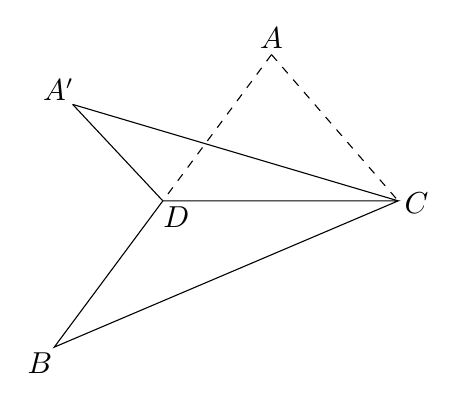
\begin{tikzpicture}[x=1pt, y=1pt,
    every node/.style={inner sep=0pt, font=\fontsize{10.5pt}{12.6pt}\selectfont}]
  \draw[line width=0.398pt] (39.2600,52.8670)   -- (0.0000,0.0000)   -- (124.3000,52.8670)   -- (39.2600,52.8670);
  \draw[line width=0.398pt] (6.6611,87.7336)   -- (39.2601,52.8666);
  \draw[line width=0.398pt] (6.6611,87.7336)   -- (124.3001,52.8666);
  \draw[line width=0.398pt, dash pattern=on 2.989pt off 2.989pt, dash phase=0.0pt] (78.5204,105.7337)   -- (39.2604,52.8667);
  \draw[line width=0.398pt, dash pattern=on 2.989pt off 2.989pt, dash phase=0.0pt] (78.5204,105.7337)   -- (124.3004,52.8667);

  \node[anchor=center] at (78.487,111.712) {$A$};  % 源中心 (610.65,351.04)
  \node[anchor=center] at (1.487,93.012) {$A'$};  % 源中心 (533.65,332.34)
  \node[anchor=center] at (130.887,51.912) {$C$};  % 源中心 (663.05,291.24)
  \node[anchor=center] at (44.087,46.962) {$D$};  % 源中心 (576.25,286.29)
  \node[anchor=center] at (-5.163,-5.888) {$B$};  % 源中心 (527.00,233.44)

\end{tikzpicture}
%
% 【自验结果】
%   探针：latexmk -pdfxe（待跑）。
\end{center}
\nopagebreak[4]
(A) \(\angle A'DB\leqslant\alpha\)　(B) \(\angle A'DB\geqslant\alpha\)　(C) \(\angle A'CB\leqslant\alpha\)　(D) \(\angle A'CB\geqslant\alpha\)

\Needspace{4\baselineskip}
\textbf{解析}

\Needspace{5\baselineskip}
以 \(D\) 为原点、直线 \(CD\) 为 \(x\) 轴、原平面为 \(z=0\) 平面建系。设
\nopagebreak[4]
\[
C=(c,0,0),\qquad B=(p,q,0)\quad(q\neq0),
\]
\Needspace{5\baselineskip}
因 \(D\) 是 \(AB\) 的中点，故
\nopagebreak[4]
\[
A=(-p,-q,0).
\]
\Needspace{5\baselineskip}
设翻折角为 \(\varphi\)，则
\nopagebreak[4]
\[
A'=(-p,-q\cos\varphi,-q\sin\varphi).
\]

\Needspace{5\baselineskip}
在过 \(D\) 且垂直于 \(CD\) 的平面内，半平面 \(BCD\) 截得射线方向 \((q,0)\)，半平面 \(A'CD\) 截得射线方向 \((-q\cos\varphi,-q\sin\varphi)\)，故二面角的平面角 \(\alpha\) 满足
\nopagebreak[4]
\[
\cos\alpha=\frac{(q,0)\cdot(-q\cos\varphi,-q\sin\varphi)}{q^2}
=-\cos\varphi.
\]

\Needspace{5\baselineskip}
又
\nopagebreak[4]
\[
\overrightarrow{DA'}\cdot\overrightarrow{DB}
=-p^2-q^2\cos\varphi=-p^2+q^2\cos\alpha,
\]
\Needspace{5\baselineskip}
且 \(|\overrightarrow{DA'}|=|\overrightarrow{DB}|=\sqrt{p^2+q^2}\)，所以
\nopagebreak[4]
\[
\cos\angle A'DB=\frac{q^2\cos\alpha-p^2}{p^2+q^2}
=\cos\alpha-\frac{p^2(1+\cos\alpha)}{p^2+q^2}\leqslant\cos\alpha.
\]
\Needspace{5\baselineskip}
余弦在 \([0,\pi]\) 上单调递减，故
\nopagebreak[4]
\[
\angle A'DB\geqslant\alpha.
\]
故 (B) 恒成立，(A) 不恒成立。

（排除 (C)(D)：取 \(p=2\)，\(q=1\)，\(c=1\)，\(\alpha=90^\circ\)，得 \(\cos\angle A'CB=-\dfrac{3}{\sqrt{20}}\)，\(\angle A'CB\approx132^\circ>\alpha\)，(C) 不成立；取 \(p=1\)，\(q=1\)，\(c=3\)，\(\alpha=90^\circ\)，得 \(\cos\angle A'CB=\dfrac{8}{\sqrt{85}}\)，\(\angle A'CB\approx30^\circ<\alpha\)，(D) 不成立。）

故选 (B)。

（验证：当 \(p=0\)（即 \(CD\perp AB\)）时 \(\cos\angle A'DB=\cos\alpha\)，取等号；当 \(\alpha\to180^\circ\) 时 \(\angle A'DB\to180^\circ\)，与平展退化情形一致。）

\gkanswer{答案：B}

\end{answer}
\begin{answer}
\gksolhead{9}{双曲线的焦距与渐近线}

\textbf{题目}：

双曲线 \(\dfrac{x^2}{2}-y^2=1\) 的焦距是\gkblank{}，渐近线方程是\gkblank{}。

\Needspace{4\baselineskip}
\textbf{解析}

\Needspace{5\baselineskip}
双曲线 \(\dfrac{x^2}{2}-y^2=1\) 中 \(a^2=2\)，\(b^2=1\)，故
\nopagebreak[4]
\[
c^2=a^2+b^2=3,\qquad c=\sqrt3.
\]
\Needspace{5\baselineskip}
焦距为
\nopagebreak[4]
\[
2c=2\sqrt3.
\]
\Needspace{5\baselineskip}
渐近线为
\nopagebreak[4]
\[
y=\pm\frac{b}{a}x=\pm\frac{1}{\sqrt2}x=\pm\frac{\sqrt2}{2}x.
\]

（验证：顶点 \((\pm\sqrt2,0)\)，焦点 \((\pm\sqrt3,0)\)；将 \(y=\dfrac{x}{\sqrt2}\) 代入方程得 \(\dfrac{x^2}{2}-\dfrac{x^2}{2}=0\)，确为渐近线。）

\gkanswer{答案：\(2\sqrt3\)；\(y=\pm\dfrac{\sqrt2}{2}x\)}

\end{answer}
\begin{answer}
\gksolhead{10}{分段函数}

\textbf{题目}：

\Needspace{5\baselineskip}
已知函数
\nopagebreak[4]
\[
f(x)=\begin{cases}
x+\dfrac{2}{x}-3, & x\geqslant1,\\
\lg\left(x^2+1\right), & x<1,
\end{cases}
\]
则 \(f(f(-3))=\)\gkblank{}，\(f(x)\) 的最小值是\gkblank{}。

\Needspace{4\baselineskip}
\textbf{解析}

\Needspace{5\baselineskip}
\(-3<1\)，故
\nopagebreak[4]
\[
f(-3)=\lg\left((-3)^2+1\right)=\lg10=1.
\]
\Needspace{5\baselineskip}
又 \(1\geqslant1\)，故
\nopagebreak[4]
\[
f(f(-3))=f(1)=1+\frac21-3=0.
\]

\Needspace{5\baselineskip}
求最小值。当 \(x\geqslant1\) 时，
\nopagebreak[4]
\[
f(x)=x+\frac2x-3\geqslant2\sqrt{x\cdot\frac2x}-3=2\sqrt2-3,
\]
等号当且仅当 \(x=\dfrac2x\)，即 \(x=\sqrt2\)（满足 \(x\geqslant1\)）。

\Needspace{5\baselineskip}
当 \(x<1\) 时，
\nopagebreak[4]
\[
f(x)=\lg\left(x^2+1\right)\geqslant\lg1=0,
\]
等号在 \(x=0\) 处取得。

\Needspace{5\baselineskip}
因 \(2\sqrt2-3<0\)，故 \(f(x)\) 的最小值为
\nopagebreak[4]
\[
2\sqrt2-3.
\]

（验证：\(2\sqrt2-3\approx-0.1716<0\)；在 \(x=\sqrt2\) 处 \(f=\sqrt2+\sqrt2-3=2\sqrt2-3\)，为第一支最小值，且小于第二支的下确界 \(0\)。）

\gkanswer{答案：\(0\)；\(2\sqrt2-3\)}

\end{answer}
\begin{answer}
\gksolhead{11}{三角恒等变换}

\textbf{题目}：

函数 \(f(x)=\sin^2x+\sin x\cos x+1\) 的最小正周期是\gkblank{}，单调递减区间是\gkblank{}。

\Needspace{4\baselineskip}
\textbf{解析}

\nopagebreak[4]
\[
f(x)=\sin^2x+\sin x\cos x+1
=\frac{1-\cos2x}{2}+\frac{\sin2x}{2}+1
=\frac32+\frac{\sqrt2}{2}\sin\left(2x-\frac{\pi}{4}\right).
\]
\Needspace{5\baselineskip}
故最小正周期
\nopagebreak[4]
\[
T=\frac{2\pi}{2}=\pi.
\]

\Needspace{5\baselineskip}
又
\nopagebreak[4]
\[
f'(x)=\sin2x+\cos2x=\sqrt2\sin\left(2x+\frac{\pi}{4}\right).
\]
\Needspace{5\baselineskip}
令 \(f'(x)\leqslant0\)，得
\nopagebreak[4]
\[
2x+\frac{\pi}{4}\in\left[\pi+2k\pi,\,2\pi+2k\pi\right],
\]
\Needspace{5\baselineskip}
即
\nopagebreak[4]
\[
x\in\left[\frac{3\pi}{8}+k\pi,\,\frac{7\pi}{8}+k\pi\right]\quad(k\in\mathbf{Z}).
\]

故最小正周期为 \(\pi\)，单调递减区间为 \(\left[\dfrac{3\pi}{8}+k\pi,\dfrac{7\pi}{8}+k\pi\right]\)（\(k\in\mathbf{Z}\)）。

（验证：\(x=\dfrac{3\pi}{8}\) 时 \(2x-\dfrac{\pi}{4}=\dfrac{\pi}{2}\)，\(f\) 取最大值 \(\dfrac32+\dfrac{\sqrt2}{2}\)；\(x=\dfrac{7\pi}{8}\) 时 \(2x-\dfrac{\pi}{4}=\dfrac{3\pi}{2}\)，\(f\) 取最小值，区间端点与递减性一致。）

\gkanswer{答案：\(\pi\)；\(\left[\dfrac{3\pi}{8}+k\pi,\dfrac{7\pi}{8}+k\pi\right]\)（\(k\in\mathbf{Z}\)）}

\end{answer}
\begin{answer}
\gksolhead{12}{对数运算}

\textbf{题目}：

若 \(a=\log_4 3\)，则 \(2^a+2^{-a}=\)\gkblank{}。

\Needspace{4\baselineskip}
\textbf{解析}

\Needspace{5\baselineskip}
由 \(a=\log_4 3=\dfrac12\log_2 3\)，得
\nopagebreak[4]
\[
2^a=2^{\frac12\log_2 3}=\sqrt3,\qquad
2^{-a}=\frac{1}{\sqrt3}=\frac{\sqrt3}{3}.
\]
\Needspace{5\baselineskip}
故
\nopagebreak[4]
\[
2^a+2^{-a}=\sqrt3+\frac{\sqrt3}{3}=\frac{4\sqrt3}{3}.
\]

（验证：\((2^a+2^{-a})^2=2^{2a}+2+2^{-2a}=3+\dfrac13+2=\dfrac{16}{3}\)，故原式为 \(\dfrac{4}{\sqrt3}=\dfrac{4\sqrt3}{3}\)。）

\gkanswer{答案：\(\dfrac{4\sqrt3}{3}\)}

\end{answer}
\begin{answer}
\gksolhead{13}{异面直线所成角}

\textbf{题目}：

如图，在三棱锥 \(A-BCD\) 中，\(AB=AC=BD=CD=3\)，\(AD=BC=2\)，点 \(M\)，\(N\) 分别为 \(AD\)，\(BC\) 的中点，则异面直线 \(AN\)，\(CM\) 所成的角的余弦值是\gkblank{}。
\nopagebreak[4]
\begin{center}% f2015zjl_q13_tetra.tex — 2015 年高考数学·浙江卷·理科 第 13 题（三棱锥与两中点）
%
% 【来源】`.work/phase3-b19/source/2015浙江理.pdf`（SHA-256
%   801150f0a6d440ac967813d264face6d48b6ee9c69cc20f1c9d6b2b38dec2e9f），
%   第 1 页（合订本页 989）；内容对象 5。逐路径实测见
%   `.work/phase3-b19/figure-inventory.md`。
%
% 【坐标口径】源 PDF 用户空间（原点左下、y 向上）。本图本地坐标
%   (x, y) = (x_page − 918.392, y_page − 615.313)，1 单位 = 1 TeX pt。
%   路径坐标逐点照录内容流（含三次贝塞尔控制点）。
%
% 元素计数：7 条路径（棱 AB/AC/AD/BC/CD 实线、BD 虚线、中线 AN/CM）＋6 个标签
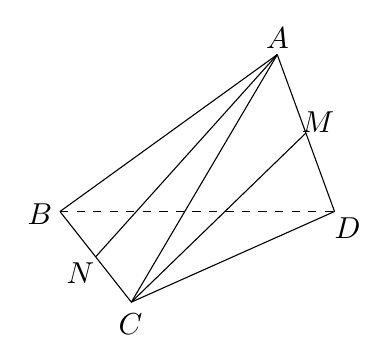
\begin{tikzpicture}[x=1pt, y=1pt,
    every node/.style={inner sep=0pt, font=\fontsize{10.5pt}{12.6pt}\selectfont}]
  \draw[line width=0.398pt] (99.2138,32.7410)   -- (78.5208,89.4350);
  \draw[line width=0.398pt] (0.0000,32.7410)   -- (25.7960,0.0000)   -- (99.2140,32.7410);
  \draw[line width=0.398pt] (78.5206,89.4346)   -- (-0.0004,32.7406);
  \draw[line width=0.398pt] (78.5206,89.4346)   -- (12.8976,16.3706);
  \draw[line width=0.398pt] (25.7957,0.0005)   -- (88.8677,61.0875);
  \draw[line width=0.398pt] (78.5206,89.4346)   -- (25.7956,0.0006);
  \draw[line width=0.398pt, dash pattern=on 2.989pt off 2.989pt, dash phase=0.0pt] (0.0000,32.7410)   -- (99.2140,32.7410);

  \node[anchor=center] at (78.558,95.427) {$A$};  % 源中心 (996.95,710.74)
  \node[anchor=center] at (93.208,65.027) {$M$};  % 源中心 (1011.60,680.34)
  \node[anchor=center] at (-7.242,31.777) {$B$};  % 源中心 (911.15,647.09)
  \node[anchor=center] at (103.958,26.827) {$D$};  % 源中心 (1022.35,642.14)
  \node[anchor=center] at (7.408,10.477) {$N$};  % 源中心 (925.80,625.79)
  \node[anchor=center] at (25.458,-7.973) {$C$};  % 源中心 (943.85,607.34)

\end{tikzpicture}
%
% 【自验结果】
%   探针：latexmk -pdfxe（待跑）。
\end{center}
\nopagebreak[4]
\Needspace{4\baselineskip}
\textbf{解析}

\Needspace{5\baselineskip}
记 \(\boldsymbol{u}=\overrightarrow{AB}\)，\(\boldsymbol{v}=\overrightarrow{AC}\)，\(\boldsymbol{w}=\overrightarrow{AD}\)。由题设 \(|\boldsymbol{u}|=|\boldsymbol{v}|=3\)，\(|\boldsymbol{w}|=2\)，且
\nopagebreak[4]
\[
|\boldsymbol{u}-\boldsymbol{v}|=2\ \Longrightarrow\ \boldsymbol{u}\cdot\boldsymbol{v}=7,
\]
\nopagebreak[4]
\[
|\boldsymbol{w}-\boldsymbol{u}|=3\ \Longrightarrow\ \boldsymbol{w}\cdot\boldsymbol{u}=2,
\]
\nopagebreak[4]
\[
|\boldsymbol{w}-\boldsymbol{v}|=3\ \Longrightarrow\ \boldsymbol{w}\cdot\boldsymbol{v}=2.
\]

\Needspace{5\baselineskip}
\(N\) 为 \(BC\) 中点，\(M\) 为 \(AD\) 中点，故
\nopagebreak[4]
\[
\overrightarrow{AN}=\frac{\boldsymbol{u}+\boldsymbol{v}}{2},\qquad
\overrightarrow{CM}=\frac{\boldsymbol{w}}{2}-\boldsymbol{v}=\frac{\boldsymbol{w}-2\boldsymbol{v}}{2}.
\]
\Needspace{5\baselineskip}
于是
\nopagebreak[4]
\[
\overrightarrow{AN}\cdot\overrightarrow{CM}
=\frac14\left(\boldsymbol{u}+\boldsymbol{v}\right)\cdot\left(\boldsymbol{w}-2\boldsymbol{v}\right)
=\frac14\left(2-14+2-18\right)=-7,
\]
\nopagebreak[4]
\[
|\overrightarrow{AN}|^2=\frac14|\boldsymbol{u}+\boldsymbol{v}|^2=\frac14(9+9+14)=8,
\]
\nopagebreak[4]
\[
|\overrightarrow{CM}|^2=\frac14|\boldsymbol{w}-2\boldsymbol{v}|^2=\frac14(4+36-4\cdot2)=8.
\]
\Needspace{5\baselineskip}
设两直线所成角为 \(\theta\in\left[0,\dfrac{\pi}{2}\right]\)，则
\nopagebreak[4]
\[
\cos\theta=\frac{|\overrightarrow{AN}\cdot\overrightarrow{CM}|}{|\overrightarrow{AN}||\overrightarrow{CM}|}
=\frac{7}{2\sqrt2\cdot2\sqrt2}=\frac78.
\]

\Needspace{5\baselineskip}
（验证：取 \(B(-1,0,0)\)，\(C(1,0,0)\)，\(N\) 为原点，令 \(A=(0,2\sqrt2,0)\)，
\nopagebreak[4]
\[
D=\left(0,\frac{3\sqrt2}{2},\frac{\sqrt{14}}{2}\right),
\]
则可逐项验证 \(AB=AC=BD=CD=3\)、\(AD=BC=2\)；再算 \(\overrightarrow{AN}\cdot\overrightarrow{CM}=7\)，两向量模长均为 \(2\sqrt2\)，同样得 \(\dfrac78\)。）

\gkanswer{答案：\(\dfrac78\)}

\end{answer}
\begin{answer}
\gksolhead{14}{绝对值函数的最值}

\textbf{题目}：

若实数 \(x\)，\(y\) 满足 \(x^2+y^2\leqslant1\)，则 \(|2x+y-2|+|6-x-3y|\) 的最小值是\gkblank{}。

\Needspace{4\baselineskip}
\textbf{解析}

\Needspace{5\baselineskip}
由 \(x^2+y^2\leqslant1\) 得
\nopagebreak[4]
\[
x+3y\leqslant\sqrt{1^2+3^2}\cdot1=\sqrt{10}<6,
\]
故 \(6-x-3y>0\) 恒成立。

\Needspace{5\baselineskip}
若 \(2x+y\geqslant2\)，则
\nopagebreak[4]
\[
|2x+y-2|+|6-x-3y|=(2x+y-2)+(6-x-3y)=x-2y+4.
\]
\Needspace{5\baselineskip}
在弦 \(2x+y=2\) 上，\(y=2-2x\)，代入 \(x^2+y^2\leqslant1\) 得 \(5x^2-8x+3\leqslant0\)，即 \(x\in\left[\dfrac35,1\right]\)，此时
\nopagebreak[4]
\[
x-2y+4=x-2(2-2x)+4=5x\geqslant3,
\]
等号在 \(x=\dfrac35\)，\(y=\dfrac45\) 处取得（该点在圆周上）。

\Needspace{5\baselineskip}
若 \(2x+y\leqslant2\)，则
\nopagebreak[4]
\[
|2x+y-2|+|6-x-3y|=(2-2x-y)+(6-x-3y)=8-3x-4y.
\]
由 \(3x+4y\leqslant5\) 得 \(8-3x-4y\geqslant3\)，等号在 \((x,y)=\left(\dfrac35,\dfrac45\right)\) 处取得。

故最小值为 \(3\)。

（验证：在 \(\left(\dfrac35,\dfrac45\right)\) 处第一项为 \(0\)，第二项为 \(6-3=3\)；再取 \((1,0)\) 得 \(5\)，\((0,1)\) 得 \(4\)，\((0,0)\) 得 \(8\)，均不小于 \(3\)。）

\gkanswer{答案：\(3\)}

\end{answer}
\begin{answer}
\gksolhead{15}{空间向量的投影}

\textbf{题目}：

已知 \(\boldsymbol{e}_1\)，\(\boldsymbol{e}_2\) 是空间单位向量，\(\boldsymbol{e}_1\cdot\boldsymbol{e}_2=\dfrac12\)，若空间向量 \(\boldsymbol{b}\) 满足 \(\boldsymbol{b}\cdot\boldsymbol{e}_1=2\)，\(\boldsymbol{b}\cdot\boldsymbol{e}_2=\dfrac52\)，且对于任意 \(x\)，\(y\in\mathbf{R}\)，\(\left|\boldsymbol{b}-(x\boldsymbol{e}_1+y\boldsymbol{e}_2)\right|\geqslant\left|\boldsymbol{b}-(x_0\boldsymbol{e}_1+y_0\boldsymbol{e}_2)\right|=1\)（\(x_0\)，\(y_0\in\mathbf{R}\)），则 \(x_0=\)\gkblank{}，\(y_0=\)\gkblank{}，\(|\boldsymbol{b}|=\)\gkblank{}。

\Needspace{4\baselineskip}
\textbf{解析}

\Needspace{5\baselineskip}
记 \(\boldsymbol{p}=x_0\boldsymbol{e}_1+y_0\boldsymbol{e}_2\)。题设不等式说明 \(\boldsymbol{p}\) 是 \(\boldsymbol{b}\) 在平面 \(\operatorname{span}\{\boldsymbol{e}_1,\boldsymbol{e}_2\}\) 上的正交投影，且 \(\left|\boldsymbol{b}-\boldsymbol{p}\right|=1\)。故 \(\boldsymbol{b}-\boldsymbol{p}\) 与 \(\boldsymbol{e}_1\)，\(\boldsymbol{e}_2\) 均垂直：
\nopagebreak[4]
\[
(\boldsymbol{b}-\boldsymbol{p})\cdot\boldsymbol{e}_1=0
\ \Longrightarrow\ x_0+\frac12y_0=2,
\]
\nopagebreak[4]
\[
(\boldsymbol{b}-\boldsymbol{p})\cdot\boldsymbol{e}_2=0
\ \Longrightarrow\ \frac12x_0+y_0=\frac52.
\]
\Needspace{5\baselineskip}
解得
\nopagebreak[4]
\[
x_0=1,\qquad y_0=2.
\]
\Needspace{5\baselineskip}
于是
\nopagebreak[4]
\[
|\boldsymbol{p}|^2=x_0^2+y_0^2+2x_0y_0(\boldsymbol{e}_1\cdot\boldsymbol{e}_2)
=1+4+2\cdot1\cdot2\cdot\frac12=7.
\]
\Needspace{5\baselineskip}
因 \(\boldsymbol{b}-\boldsymbol{p}\perp\boldsymbol{p}\)，
\nopagebreak[4]
\[
|\boldsymbol{b}|^2=|\boldsymbol{p}|^2+|\boldsymbol{b}-\boldsymbol{p}|^2=7+1=8,
\]
\Needspace{5\baselineskip}
故
\nopagebreak[4]
\[
|\boldsymbol{b}|=2\sqrt2.
\]

（验证：\(\boldsymbol{p}=\boldsymbol{e}_1+2\boldsymbol{e}_2\)，\(\boldsymbol{p}\cdot\boldsymbol{e}_1=1+1=2\)，\(\boldsymbol{p}\cdot\boldsymbol{e}_2=\dfrac12+2=\dfrac52\)，与 \(\boldsymbol{b}\) 的两个内积一致；对任意 \(x,y\)，\(|\boldsymbol{b}-(x\boldsymbol{e}_1+y\boldsymbol{e}_2)|^2=|\boldsymbol{b}-\boldsymbol{p}|^2+|\boldsymbol{p}-(x\boldsymbol{e}_1+y\boldsymbol{e}_2)|^2\geqslant1\)，仅当 \(x=x_0\)，\(y=y_0\) 时取等。）

\gkanswer{答案：\(x_0=1\)，\(y_0=2\)，\(|\boldsymbol{b}|=2\sqrt2\)}

\end{answer}
\begin{answer}
\gksolhead{16}{解三角形}

\textbf{题目}：

在 \(\triangle ABC\) 中，内角 \(A\)，\(B\)，\(C\) 所对的边分别是 \(a\)，\(b\)，\(c\)。已知 \(A=\dfrac{\pi}{4}\)，\(b^2-a^2=\dfrac12c^2\)。

（1） 求 \(\tan C\) 的值；

（2） 若 \(\triangle ABC\) 的面积为 \(3\)，求 \(b\) 的值。

\Needspace{4\baselineskip}
\textbf{解析}

\gksubpart{(1)}

\Needspace{5\baselineskip}
由余弦定理，
\nopagebreak[4]
\[
a^2=b^2+c^2-2bc\cos A=b^2+c^2-\sqrt2bc.
\]
\Needspace{5\baselineskip}
代入 \(b^2-a^2=\dfrac12c^2\) 得
\nopagebreak[4]
\[
\sqrt2bc-c^2=\frac12c^2
\ \Longrightarrow\ \sqrt2b=\frac32c
\ \Longrightarrow\ b=\frac{3\sqrt2}{4}c.
\]
\Needspace{5\baselineskip}
由正弦定理 \(\dfrac{b}{\sin B}=\dfrac{c}{\sin C}\)，得
\nopagebreak[4]
\[
\sin B=\frac{3\sqrt2}{4}\sin C.
\]
\Needspace{5\baselineskip}
又 \(B=\dfrac{3\pi}{4}-C\)，故
\nopagebreak[4]
\[
\sin\left(\frac{3\pi}{4}-C\right)=\frac{\sqrt2}{2}(\cos C+\sin C),
\]
\Needspace{5\baselineskip}
从而
\nopagebreak[4]
\[
\frac{\sqrt2}{2}(\cos C+\sin C)=\frac{3\sqrt2}{4}\sin C
\ \Longrightarrow\ \cos C=\frac12\sin C
\ \Longrightarrow\ \tan C=2.
\]

\gksubpart{(2)}

\Needspace{5\baselineskip}
面积
\nopagebreak[4]
\[
S=\frac12bc\sin A=\frac12bc\cdot\frac{\sqrt2}{2}=3
\ \Longrightarrow\ bc=6\sqrt2.
\]
\Needspace{5\baselineskip}
又 \(b=\dfrac{3\sqrt2}{4}c\)，代入得
\nopagebreak[4]
\[
\frac{3\sqrt2}{4}c^2=6\sqrt2
\ \Longrightarrow\ c^2=8,\qquad c=2\sqrt2.
\]
\Needspace{5\baselineskip}
于是
\nopagebreak[4]
\[
b=\frac{3\sqrt2}{4}\cdot2\sqrt2=3.
\]

（验证：\(b=3\)，\(c=2\sqrt2\) 时 \(a^2=9+8-12=5\)，\(a=\sqrt5\)，\(b^2-a^2=4=\dfrac12c^2\)；\(\sin C=\dfrac{c\sin A}{a}=\dfrac{2}{\sqrt5}\)，\(\cos C=\dfrac{1}{\sqrt5}\)，\(\tan C=2\)；面积 \(\dfrac12\cdot3\cdot2\sqrt2\cdot\dfrac{\sqrt2}{2}=3\)，三处自洽。）

\gkanswer{答案（1）：\(2\)。}

\gkanswer{答案（2）：\(3\)。}

\end{answer}
\begin{answer}
\gksolhead{17}{三棱柱中的线面垂直与二面角}

\textbf{题目}：

如图，在三棱柱 \(ABC-A_1B_1C_1\) 中，\(\angle BAC=90^\circ\)，\(AB=AC=2\)，\(A_1A=4\)，\(A_1\) 在底面 \(ABC\) 的射影为 \(BC\) 的中点，\(D\) 是 \(B_1C_1\) 的中点。

（1） 证明：\(A_1D\perp\) 平面 \(A_1BC\)；

（2） 求二面角 \(A_1-BD-B_1\) 的平面角的余弦值。
\nopagebreak[4]
\begin{center}% f2015zjl_q17_prism.tex — 2015 年高考数学·浙江卷·理科 第 17 题（三棱柱）
%
% 【来源】`.work/phase3-b19/source/2015浙江理.pdf`（SHA-256
%   801150f0a6d440ac967813d264face6d48b6ee9c69cc20f1c9d6b2b38dec2e9f），
%   第 2 页（合订本页 990）；内容对象 23。逐路径实测见
%   `.work/phase3-b19/figure-inventory.md`。
%
% 【坐标口径】源 PDF 用户空间（原点左下、y 向上）。本图本地坐标
%   (x, y) = (x_page − 259.718, y_page − 561.951)，1 单位 = 1 TeX pt。
%   路径坐标逐点照录内容流（含三次贝塞尔控制点）。
%
% 元素计数：13 条路径（8 实＋5 虚）＋7 个标签
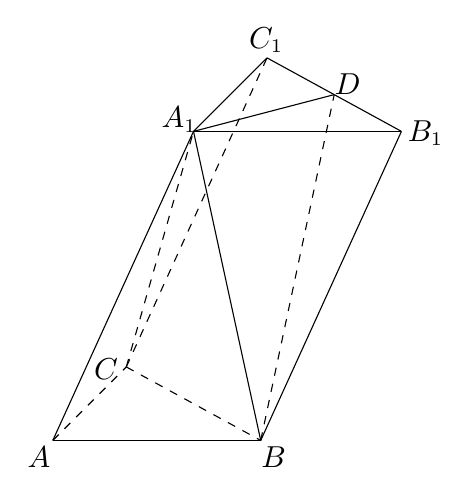
\begin{tikzpicture}[x=1pt, y=1pt,
    every node/.style={inner sep=0pt, font=\fontsize{10.5pt}{12.6pt}\selectfont}]
  \draw[line width=0.3985pt] (0.0000,0.0000)   (0.0000,0.0000)   -- (75.1352,0.0000);
  \draw[line width=0.3985pt] (75.1352,0.0000)   (75.1352,0.0000)   -- (50.8477,111.6752);
  \draw[line width=0.3985pt] (50.8477,111.6752)   (50.8477,111.6752)   -- (125.9829,111.6752);
  \draw[line width=0.3985pt] (125.9829,111.6752)   (125.9829,111.6752)   -- (77.4080,138.2355);
  \draw[line width=0.3985pt] (77.4080,138.2355)   (77.4080,138.2355)   -- (50.8477,111.6752);
  \draw[line width=0.3985pt] (75.1352,0.0000)   (75.1352,0.0000)   -- (125.9829,111.6752);
  \draw[line width=0.3985pt] (0.0000,0.0000)   (0.0000,0.0000)   -- (50.8477,111.6752);
  \draw[line width=0.3985pt] (101.6955,124.9553)   (101.6955,124.9553)   -- (50.8477,111.6752);
  \draw[line width=0.3985pt, dash pattern=on 2.98883pt off 2.98883pt, dash phase=0.0pt] (75.1352,0.0000)   (75.1352,0.0000)   -- (101.6955,124.9553);
  \draw[line width=0.3985pt, dash pattern=on 2.98883pt off 2.98883pt, dash phase=0.0pt] (0.0000,0.0000)   (0.0000,0.0000)   -- (26.5603,26.5603);
  \draw[line width=0.3985pt, dash pattern=on 2.98883pt off 2.98883pt, dash phase=0.0pt] (26.5603,26.5603)   (26.5603,26.5603)   -- (77.4080,138.2355);
  \draw[line width=0.3985pt, dash pattern=on 2.98883pt off 2.98883pt, dash phase=0.0pt] (26.5603,26.5603)   (26.5603,26.5603)   -- (50.8477,111.6752);
  \draw[line width=0.3985pt, dash pattern=on 2.98883pt off 2.98883pt, dash phase=0.0pt] (26.5603,26.5603)   (26.5603,26.5603)   -- (75.1352,0.0000);

  \node[anchor=center] at (77.132,144.589) {$C_1$};  % 源中心 (336.85,706.54)
  \node[anchor=center] at (106.482,128.889) {$D$};  % 源中心 (366.20,690.84)
  \node[anchor=center] at (45.682,115.989) {$A_1$};  % 源中心 (305.40,677.94)
  \node[anchor=center] at (134.682,111.039) {$B_1$};  % 源中心 (394.40,672.99)
  \node[anchor=center] at (19.232,25.589) {$C$};  % 源中心 (278.95,587.54)
  \node[anchor=center] at (-4.968,-5.911) {$A$};  % 源中心 (254.75,556.04)
  \node[anchor=center] at (79.782,-5.911) {$B$};  % 源中心 (339.50,556.04)

\end{tikzpicture}
%
% 【自验结果】
%   探针：latexmk -pdfxe（待跑）。
\end{center}
\nopagebreak[4]
\Needspace{4\baselineskip}
\textbf{解析}

\gksubpart{(1)}

\Needspace{5\baselineskip}
取 \(A\) 为原点，\(AB\) 为 \(x\) 轴、\(AC\) 为 \(y\) 轴建系：
\nopagebreak[4]
\[
A(0,0,0),\quad B(2,0,0),\quad C(0,2,0).
\]
\Needspace{5\baselineskip}
\(BC\) 的中点为 \(O(1,1,0)\)，\(AO=\sqrt2\)。设 \(A_1=(1,1,h)\)，由 \(A_1A=4\) 得
\nopagebreak[4]
\[
h=\sqrt{16-2}=\sqrt{14},
\]
\Needspace{5\baselineskip}
故
\nopagebreak[4]
\[
A_1(1,1,\sqrt{14}).
\]
\Needspace{5\baselineskip}
棱柱平移向量为 \(\overrightarrow{AA_1}=(1,1,\sqrt{14})\)，于是
\nopagebreak[4]
\[
B_1(3,1,\sqrt{14}),\qquad C_1(1,3,\sqrt{14}),\qquad D(2,2,\sqrt{14}).
\]
\nopagebreak[4]
\[
\overrightarrow{A_1D}=(1,1,0),\quad
\overrightarrow{A_1B}=(1,-1,-\sqrt{14}),\quad
\overrightarrow{A_1C}=(-1,1,-\sqrt{14}).
\]
\nopagebreak[4]
\[
\overrightarrow{A_1D}\cdot\overrightarrow{A_1B}=1-1+0=0,\qquad
\overrightarrow{A_1D}\cdot\overrightarrow{A_1C}=-1+1+0=0.
\]
\Needspace{5\baselineskip}
故 \(A_1D\) 垂直于平面 \(A_1BC\) 内两条相交直线 \(A_1B\)，\(A_1C\)，从而
\nopagebreak[4]
\[
A_1D\perp\text{平面 }A_1BC.
\]

\gksubpart{(2)}

\Needspace{5\baselineskip}
平面 \(A_1BD\) 的法向量
\nopagebreak[4]
\[
\boldsymbol{n}_1=\overrightarrow{BA_1}\times\overrightarrow{BD}
=(-1,1,\sqrt{14})\times(0,2,\sqrt{14})
=(-\sqrt{14},\sqrt{14},-2).
\]
\Needspace{5\baselineskip}
平面 \(BDB_1\) 的法向量
\nopagebreak[4]
\[
\boldsymbol{n}_2=\overrightarrow{BD}\times\overrightarrow{BB_1}
=(0,2,\sqrt{14})\times(1,1,\sqrt{14})
=(\sqrt{14},\sqrt{14},-2).
\]
\Needspace{5\baselineskip}
于是
\nopagebreak[4]
\[
\boldsymbol{n}_1\cdot\boldsymbol{n}_2=-14+14+4=4,\qquad
|\boldsymbol{n}_1|=|\boldsymbol{n}_2|=\sqrt{32},
\]
\Needspace{5\baselineskip}
两平面所成锐角的余弦为
\nopagebreak[4]
\[
\frac{4}{32}=\frac18.
\]

\Needspace{5\baselineskip}
判定二面角的平面角是钝角还是锐角。在棱 \(BD\) 上取点 \(B\)，作两个半平面内垂直于 \(BD\) 的射线：
\nopagebreak[4]
\[
\boldsymbol{u}_1=\overrightarrow{BA_1}-\frac{\overrightarrow{BA_1}\cdot\overrightarrow{BD}}{|\overrightarrow{BD}|^2}\overrightarrow{BD}
=\left(-1,-\frac79,\frac{\sqrt{14}}{9}\right),
\]
\nopagebreak[4]
\[
\boldsymbol{u}_2=\overrightarrow{BB_1}-\frac{\overrightarrow{BB_1}\cdot\overrightarrow{BD}}{|\overrightarrow{BD}|^2}\overrightarrow{BD}
=\left(1,-\frac79,\frac{\sqrt{14}}{9}\right).
\]
\Needspace{5\baselineskip}
因
\nopagebreak[4]
\[
\boldsymbol{u}_1\cdot\boldsymbol{u}_2=-1+\frac{49}{81}+\frac{14}{81}
=-\frac29,\qquad
|\boldsymbol{u}_1|^2=|\boldsymbol{u}_2|^2=\frac{16}{9},
\]
\Needspace{5\baselineskip}
故平面角的余弦为
\nopagebreak[4]
\[
\frac{-\frac29}{\frac{16}{9}}=-\frac18.
\]
即二面角 \(A_1-BD-B_1\) 的平面角的余弦值为 \(-\dfrac18\)。

（验证：\(\overrightarrow{A_1D}\cdot\overrightarrow{A_1B}=\overrightarrow{A_1D}\cdot\overrightarrow{A_1C}=0\) 直接验证线面垂直；换基点 \(D\) 复算投影向量，仍得 \(\boldsymbol{u}_1=\left(-1,-\dfrac79,\dfrac{\sqrt{14}}{9}\right)\)，\(\boldsymbol{u}_2=\left(1,-\dfrac79,\dfrac{\sqrt{14}}{9}\right)\)，余弦为 \(-\dfrac18\)。若只取两法向量夹角的锐角，则得 \(\dfrac18\)，与平面角为钝角互补。）

\gkanswer{答案（1）：成立（建系得 \(\overrightarrow{A_1D}\) 与平面 \(A_1BC\) 内两条相交直线 \(A_1B\)、\(A_1C\) 均垂直）。}

\gkanswer{答案（2）：\(-\dfrac18\)。}

\end{answer}
\begin{answer}
\gksolhead{18}{二次函数的最大值}

\textbf{题目}：

\looseness=-1 已知函数 \(f(x)=x^2+ax+b\)（\(a,b\in\mathbf{R}\)），记 \(M(a,b)\) 是 \(|f(x)|\) 在区间 \([-1,1]\) 上的最大值。

（1） 证明：当 \(|a|\geqslant2\) 时，\(M(a,b)\geqslant2\)；

（2） 当 \(a\)，\(b\) 满足 \(M(a,b)\leqslant2\) 时，求 \(|a|+|b|\) 的最大值。

\Needspace{4\baselineskip}
\textbf{解析}

\gksubpart{(1)}

\Needspace{5\baselineskip}
因 \(M(a,b)\) 是 \(|f(x)|\) 在 \([-1,1]\) 上的最大值，
\nopagebreak[4]
\[
M(a,b)\geqslant\max\{|f(1)|,|f(-1)|\}
\geqslant\frac12|f(1)-f(-1)|
=\frac12|2a|=|a|.
\]
\Needspace{5\baselineskip}
当 \(|a|\geqslant2\) 时，
\nopagebreak[4]
\[
M(a,b)\geqslant|a|\geqslant2.
\]

\gksubpart{(2)}

由 (1) 知 \(M(a,b)\geqslant|a|\)，故当 \(M(a,b)\leqslant2\) 时 \(|a|\leqslant2\)。

又 \(f(-x)=x^2-ax+b\)，在 \(x\mapsto-x\) 下 \(a\) 变号而 \(b\) 与 \(M\) 不变，故不妨设 \(a\geqslant0\)，只需最大化 \(a+|b|\)。

\Needspace{5\baselineskip}
由 \(|f(1)|\leqslant2\) 得
\nopagebreak[4]
\[
-2\leqslant1+a+b\leqslant2
\ \Longrightarrow\ -3-a\leqslant b\leqslant1-a,
\]
\Needspace{5\baselineskip}
由 \(|f(-1)|\leqslant2\) 得
\nopagebreak[4]
\[
-2\leqslant1-a+b\leqslant2
\ \Longrightarrow\ a-3\leqslant b\leqslant a+1.
\]
\Needspace{5\baselineskip}
因 \(a\geqslant0\)，两区间之交为
\nopagebreak[4]
\[
a-3\leqslant b\leqslant1-a.
\]
\Needspace{5\baselineskip}
若 \(b\geqslant0\)，则
\nopagebreak[4]
\[
a+|b|=a+b\leqslant a+(1-a)=1;
\]
\Needspace{5\baselineskip}
若 \(b<0\)，则
\nopagebreak[4]
\[
a+|b|=a-b\leqslant a-(a-3)=3.
\]
\Needspace{5\baselineskip}
故
\nopagebreak[4]
\[
|a|+|b|\leqslant3.
\]
\Needspace{5\baselineskip}
当 \(a=2\)，\(b=-1\) 时，\(b=a-3=1-a\)，两处同时取等。此时
\nopagebreak[4]
\[
f(x)=x^2+2x-1,
\]
在 \([-1,1]\) 上单调递增，\(f(-1)=-2\)，\(f(1)=2\)，故 \(M(2,-1)=2\)，满足条件，且 \(|a|+|b|=3\)。由对称性 \((a,b)=(-2,-1)\) 也可。故最大值为 \(3\)。

（验证：取 \(a=\dfrac32\)，端点约束给 \(b\in\left[-\dfrac32,-\dfrac12\right]\)，但顶点值 \(f\left(-\dfrac34\right)=b-\dfrac{9}{16}\) 须满足 \(|f|\leqslant2\)，即 \(b\geqslant-\dfrac{23}{16}\)，于是 \(a+|b|\leqslant\dfrac32+\dfrac{23}{16}=\dfrac{47}{16}<3\)，未达上界。）

\gkanswer{答案（1）：成立（\(M(a,b)\geqslant\max\{|f(1)|,|f(-1)|\}\geqslant\dfrac12|f(1)-f(-1)|=|a|\geqslant2\)）。}

\gkanswer{答案（2）：\(3\)。}

\end{answer}
\begin{answer}
\gksolhead{19}{椭圆与对称弦}

\textbf{题目}：

已知椭圆 \(\dfrac{x^2}{2}+y^2=1\) 上两个不同的点 \(A\)，\(B\) 关于直线 \(y=mx+\dfrac12\) 对称。

（1） 求实数 \(m\) 的取值范围；

（2） 求 \(\triangle AOB\) 面积的最大值（\(O\) 为坐标原点）。
\nopagebreak[4]
\begin{center}% f2015zjl_q19_ellipse.tex — 2015 年高考数学·浙江卷·理科 第 19 题（椭圆与对称弦）
%
% 【来源】`.work/phase3-b19/source/2015浙江理.pdf`（SHA-256
%   801150f0a6d440ac967813d264face6d48b6ee9c69cc20f1c9d6b2b38dec2e9f），
%   第 2 页（合订本页 990）；内容对象 23。逐路径实测见
%   `.work/phase3-b19/figure-inventory.md`。
%
% 【坐标口径】源 PDF 用户空间（原点左下、y 向上）。本图本地坐标
%   (x, y) = (x_page − 599.627, y_page − 586.119)，1 单位 = 1 TeX pt。
%   路径坐标逐点照录内容流（含三次贝塞尔控制点）。
%
% 元素计数：9 条路径（x/y 轴＋箭头、椭圆、对称轴、OA/OB/AB）＋5 个标签
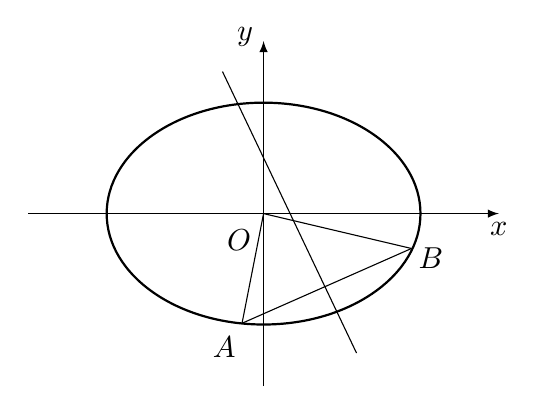
\begin{tikzpicture}[x=1pt, y=1pt,
    every node/.style={inner sep=0pt, font=\fontsize{10.5pt}{12.6pt}\selectfont}]
  \draw[line width=0.3985pt] (-0.0004,62.3630)   -- (166.4939,62.3630);
  \fill[line width=0.3985pt] (170.0804,62.3630)   .. controls (169.0177,62.5622) and (167.2909,63.1600) .. (166.0954,63.8574)   -- (166.0954,60.8686)   .. controls (167.2909,61.5660) and (169.0177,62.1637) .. (170.0804,62.3630);
  \draw[line width=0.3985pt] (85.0400,0.0001)   -- (85.0400,121.1393);
  \fill[line width=0.3985pt] (85.0400,124.7259)   .. controls (84.8408,123.6632) and (84.2430,121.9363) .. (83.5456,120.7408)   -- (86.5344,120.7408)   .. controls (85.8370,121.9363) and (85.2393,123.6632) .. (85.0400,124.7259);
  \draw[line width=0.79701pt] (85.0400,62.3630)   (141.7336,62.3630)   .. controls (141.7336,84.5002) and (116.3514,102.4454) .. (85.0400,102.4454)   .. controls (53.7286,102.4454) and (28.3464,84.5002) .. (28.3464,62.3630)   .. controls (28.3464,40.2258) and (53.7286,22.2806) .. (85.0400,22.2806)   .. controls (116.3514,22.2806) and (141.7336,40.2258) .. (141.7336,62.3630)   -- cycle   (85.0400,62.3630);
  \draw[line width=0.3985pt] (85.0400,62.3630)   -- (138.4822,49.7545);
  \draw[line width=0.3985pt] (85.0400,62.3630)   -- (77.2617,22.7287);
  \draw[line width=0.3985pt] (118.6253,11.9736)   -- (70.1862,113.6905);
  \draw[line width=0.3985pt] (77.2617,22.7287)   -- (138.4822,49.7545);

  \node[anchor=center] at (78.373,126.121) {$y$};  % 源中心 (678.00,712.24)
  \node[anchor=center] at (76.173,52.721) {$O$};  % 源中心 (675.80,638.84)
  \node[anchor=center] at (70.873,13.921) {$A$};  % 源中心 (670.50,600.04)
  \node[anchor=center] at (170.073,56.771) {$x$};  % 源中心 (769.70,642.89)
  \node[anchor=center] at (145.473,46.371) {$B$};  % 源中心 (745.10,632.49)

\end{tikzpicture}
%
% 【自验结果】
%   探针：latexmk -pdfxe（待跑）。
\end{center}
\nopagebreak[4]
\Needspace{4\baselineskip}
\textbf{解析}

\gksubpart{(1)}

设 \(AB\) 的斜率为 \(k\)。因 \(A\)，\(B\) 关于直线 \(y=mx+\dfrac12\) 对称，故 \(AB\) 与该直线垂直，\(k=-\dfrac1m\)（\(m\neq0\)；\(m=0\) 时对称轴为水平线，而椭圆上关于水平线对称的两点连线为竖直线，其中点在 \(x\) 轴上，不可能落在 \(y=\dfrac12\) 上，无解）。

\Needspace{5\baselineskip}
设
\nopagebreak[4]
\[
AB:\ y=-\frac{x}{m}+n.
\]
\Needspace{5\baselineskip}
代入椭圆方程 \(\dfrac{x^2}{2}+y^2=1\)，得
\nopagebreak[4]
\[
\left(1+\frac{2}{m^2}\right)x^2-\frac{4n}{m}x+2n^2-2=0.
\]
\Needspace{5\baselineskip}
设 \(A(x_1,y_1)\)，\(B(x_2,y_2)\)，由韦达定理，
\nopagebreak[4]
\[
x_1+x_2=\frac{4nm}{m^2+2}.
\]
\Needspace{5\baselineskip}
中点 \(P\) 的坐标为
\nopagebreak[4]
\[
x_P=\frac{2nm}{m^2+2},\qquad
y_P=n-\frac{x_P}{m}=\frac{nm^2}{m^2+2}.
\]
\Needspace{5\baselineskip}
因 \(P\) 在对称轴上，
\nopagebreak[4]
\[
\frac{nm^2}{m^2+2}=m\cdot\frac{2nm}{m^2+2}+\frac12
\ \Longrightarrow\ -\frac{nm^2}{m^2+2}=\frac12
\ \Longrightarrow\ n=-\frac{m^2+2}{2m^2}.
\]
\Needspace{5\baselineskip}
方程有两相异实根，故判别式
\nopagebreak[4]
\[
\Delta=\left(\frac{4n}{m}\right)^2-4\left(1+\frac{2}{m^2}\right)(2n^2-2)
=8\left(1+\frac{2}{m^2}-n^2\right)>0.
\]
\Needspace{5\baselineskip}
代入 \(n\) 得
\nopagebreak[4]
\[
1+\frac{2}{m^2}-\frac{(m^2+2)^2}{4m^4}>0
\ \Longrightarrow\ (m^2+2)^2<4m^2(m^2+2)
\ \Longrightarrow\ m^2>\frac23.
\]
\Needspace{5\baselineskip}
故
\nopagebreak[4]
\[
m\in\left(-\infty,-\frac{\sqrt6}{3}\right)\cup\left(\frac{\sqrt6}{3},+\infty\right).
\]

\gksubpart{(2)}

\Needspace{5\baselineskip}
\(O\) 到直线 \(AB\) 的距离
\nopagebreak[4]
\[
d=\frac{|n|}{\sqrt{1+\frac{1}{m^2}}}
=\frac{|n||m|}{\sqrt{m^2+1}},
\]
\Needspace{5\baselineskip}
又
\nopagebreak[4]
\[
|AB|=\sqrt{1+\frac{1}{m^2}}\,|x_1-x_2|.
\]
\Needspace{5\baselineskip}
故
\nopagebreak[4]
\[
S_{\triangle AOB}=\frac12|AB|d=\frac12|n||x_1-x_2|.
\]
\Needspace{5\baselineskip}
记 \(t=m^2>\dfrac23\)。由
\nopagebreak[4]
\[
|x_1-x_2|=\frac{\sqrt\Delta}{1+\frac{2}{m^2}}
=\frac{\sqrt{8\left(1+\frac{2}{t}-n^2\right)}}{\frac{t+2}{t}}
=\frac{\sqrt2\sqrt{3t^2+4t-4}}{t+2},
\]
\Needspace{5\baselineskip}
其中用到
\nopagebreak[4]
\[
1+\frac{2}{t}-\frac{(t+2)^2}{4t^2}
=\frac{3t^2+4t-4}{4t^2},
\]
\Needspace{5\baselineskip}
且 \(|n|=\dfrac{t+2}{2t}\)，所以
\nopagebreak[4]
\[
S=\frac12\cdot\frac{t+2}{2t}\cdot\frac{\sqrt2\sqrt{3t^2+4t-4}}{t+2}
=\frac{\sqrt2}{4t}\sqrt{3t^2+4t-4}.
\]
\Needspace{5\baselineskip}
于是
\nopagebreak[4]
\[
S^2=\frac{3t^2+4t-4}{8t^2}
=\frac18\left(3+\frac4t-\frac4{t^2}\right).
\]
\Needspace{5\baselineskip}
令 \(u=\dfrac1t\)，则
\nopagebreak[4]
\[
S^2=\frac18\left(3+4u-4u^2\right)
=\frac18\left(4-4\left(u-\frac12\right)^2\right),
\]
\Needspace{5\baselineskip}
当 \(u=\dfrac12\)（即 \(t=2\)）时取最大值
\nopagebreak[4]
\[
S^2=\frac12,\qquad S=\frac{\sqrt2}{2}.
\]
\(t=2>\dfrac23\)，可以取到。故 \(\triangle AOB\) 面积的最大值为 \(\dfrac{\sqrt2}{2}\)。

（验证：取 \(m=\sqrt2\)，则 \(n=-1\)，\(AB:y=-\dfrac{x}{\sqrt2}-1\)。代入椭圆得 \(x(x+\sqrt2)=0\)，\(A(-\sqrt2,0)\)，\(B(0,-1)\)，其中点 \(\left(-\dfrac{\sqrt2}{2},-\dfrac12\right)\) 在对称轴 \(y=\sqrt2x+\dfrac12\) 上；面积 \(S=\dfrac12\cdot\sqrt2=\dfrac{\sqrt2}{2}\)，达到最大值。）

\gkanswer{答案（1）：\(m\in\left(-\infty,-\dfrac{\sqrt6}{3}\right)\cup\left(\dfrac{\sqrt6}{3},+\infty\right)\)。}

\gkanswer{答案（2）：\(\dfrac{\sqrt2}{2}\)。}

\end{answer}
\begin{answer}
\gksolhead{20}{数列不等式}

\textbf{题目}：

已知数列 \(\{a_n\}\) 满足 \(a_1=\dfrac12\) 且 \(a_{n+1}=a_n-a_n^2\)（\(n\in\mathbf{N}^*\)）。

（1） 证明：\(1\leqslant\dfrac{a_n}{a_{n+1}}\leqslant2\)（\(n\in\mathbf{N}^*\)）；

（2） 设数列 \(\{a_n^2\}\) 的前 \(n\) 项和为 \(S_n\)，证明：\(\dfrac{1}{2(n+2)}\leqslant\dfrac{S_n}{n}\leqslant\dfrac{1}{2(n+1)}\)（\(n\in\mathbf{N}^*\)）。

\Needspace{4\baselineskip}
\textbf{解析}

\Needspace{5\baselineskip}
先证
\nopagebreak[4]
\[
0<a_n\leqslant\frac12\quad(n\in\mathbf{N}^*).
\]
\Needspace{5\baselineskip}
\(n=1\) 时 \(a_1=\dfrac12\)。若 \(0<a_n\leqslant\dfrac12\)，则
\nopagebreak[4]
\[
a_{n+1}=a_n(1-a_n),
\]
\Needspace{5\baselineskip}
其中 \(1-a_n\in\left[\dfrac12,1\right)\)，故 \(a_{n+1}>0\) 且
\nopagebreak[4]
\[
a_{n+1}\leqslant\frac12\cdot\frac12=\frac14<\frac12.
\]
归纳得 \(0<a_n\leqslant\dfrac12\)，且 \(n\geqslant2\) 时 \(a_n\leqslant\dfrac14\)。

\gksubpart{(1)}

\Needspace{5\baselineskip}
因 \(a_{n+1}=a_n(1-a_n)\) 且 \(a_n>0\)，故
\nopagebreak[4]
\[
\frac{a_n}{a_{n+1}}=\frac{1}{1-a_n}.
\]
\Needspace{5\baselineskip}
由 \(0<a_n\leqslant\dfrac12\) 得 \(1-a_n\in\left[\dfrac12,1\right)\)，故
\nopagebreak[4]
\[
1\leqslant\frac{1}{1-a_n}\leqslant2,
\]
\Needspace{5\baselineskip}
即
\nopagebreak[4]
\[
1\leqslant\frac{a_n}{a_{n+1}}\leqslant2\quad(n\in\mathbf{N}^*).
\]

\gksubpart{(2)}

\Needspace{5\baselineskip}
由递推式得恒等式
\nopagebreak[4]
\[
a_k^2=a_k-a_{k+1},
\]
\Needspace{5\baselineskip}
故
\nopagebreak[4]
\[
S_n=\sum_{k=1}^n a_k^2=\sum_{k=1}^n\left(a_k-a_{k+1}\right)
=a_1-a_{n+1}=\frac12-a_{n+1}.
\]
\Needspace{5\baselineskip}
于是所证不等式等价于
\nopagebreak[4]
\[
\frac{1}{2(n+1)}\leqslant a_{n+1}\leqslant\frac{1}{n+2}.
\]
\Needspace{5\baselineskip}
下面证明：对一切 \(k\geqslant2\)，
\nopagebreak[4]
\[
\frac{1}{2k}\leqslant a_k\leqslant\frac{1}{k+1}.
\]
\(k=2\) 时 \(a_2=\dfrac12\left(1-\dfrac12\right)=\dfrac14\)，而 \(\dfrac14\leqslant\dfrac14\leqslant\dfrac13\)，成立。

\Needspace{5\baselineskip}
设结论对 \(k\) 成立。函数 \(g(x)=x(1-x)\) 在 \(\left[0,\dfrac12\right]\) 上单调递增，且 \(a_k\leqslant\dfrac{1}{k+1}\leqslant\dfrac12\)，故
\nopagebreak[4]
\[
a_{k+1}=g(a_k)\geqslant g\left(\frac{1}{2k}\right)
=\frac{1}{2k}\left(1-\frac{1}{2k}\right)
=\frac{2k-1}{4k^2}.
\]
\Needspace{5\baselineskip}
而
\nopagebreak[4]
\[
\frac{2k-1}{4k^2}\geqslant\frac{1}{2(k+1)}
\iff(2k-1)(k+1)\geqslant2k^2
\iff k\geqslant1,
\]
\Needspace{5\baselineskip}
故左半不等式成立。又
\nopagebreak[4]
\[
a_{k+1}=g(a_k)\leqslant g\left(\frac{1}{k+1}\right)
=\frac{k}{(k+1)^2},
\]
\Needspace{5\baselineskip}
而
\nopagebreak[4]
\[
\frac{k}{(k+1)^2}\leqslant\frac{1}{k+2}
\iff k(k+2)\leqslant(k+1)^2
\iff0\leqslant1,
\]
故右半不等式也成立。归纳完成。

\Needspace{5\baselineskip}
取 \(k=n+1\geqslant2\)，得
\nopagebreak[4]
\[
\frac{1}{2(n+1)}\leqslant a_{n+1}\leqslant\frac{1}{n+2}.
\]
\Needspace{5\baselineskip}
代入 \(S_n=\dfrac12-a_{n+1}\) 即得
\nopagebreak[4]
\[
\frac{1}{2(n+2)}\leqslant\frac{S_n}{n}\leqslant\frac{1}{2(n+1)}
\quad(n\in\mathbf{N}^*).
\]

（验证：\(n=1\) 时 \(S_1=\dfrac14\)，\(\dfrac{S_1}{1}=\dfrac14\)，而 \(\dfrac16\leqslant\dfrac14\leqslant\dfrac14\)，右端取等；\(n=2\) 时 \(S_2=\dfrac{5}{16}\)，\(\dfrac{S_2}{2}=\dfrac{5}{32}\)，而 \(\dfrac18\leqslant\dfrac{5}{32}\leqslant\dfrac16\)；\(n=3\) 时 \(S_3=\dfrac{89}{256}\)，\(\dfrac{S_3}{3}=\dfrac{89}{768}\)，而 \(\dfrac{1}{10}\leqslant\dfrac{89}{768}\leqslant\dfrac18\)。逐项与恒等式 \(a_k^2=a_k-a_{k+1}\) 相符。）

\gkanswer{答案（1）：成立（\(\dfrac{a_n}{a_{n+1}}=\dfrac{1}{1-a_n}\)，由 \(0<a_n\leqslant\dfrac12\) 得 \(\dfrac{1}{1-a_n}\in[1,2)\)）。}

\gkanswer{答案（2）：成立（\(S_n=\dfrac12-a_{n+1}\)，结合 \(\dfrac{1}{2k}\leqslant a_k\leqslant\dfrac{1}{k+1}\)（\(k\geqslant2\)）即得）。}

\end{answer}